\chapter{Near hole routing protocol}\label{chapter4}
In this chapter, we describe our near hole routing protocol in details. 
\section{Proposed Scheme}
\subsection{Assumptions and definitions}
To ease the comprehension, we present a short overview of terms and definitions related to routing holes. Following the approach in \cite{ehds,elbar,issnip}, we consider the same assumptions as follows.
\begin{itemize}
\item Each node knows the position of itself and its 1-hop neighbors by using GPS or other positioning services.
\item The location of a destination is known by a source.
\item All the sensor nodes have the same radio hardware. Let $R_c$ denote the transmission range of a node.
\item The energy consumption of the computation performed for one packet at a node is negligible compared to the energy consumption of the transmission of one packet.
\end{itemize}
We start with the definitions of the notations and terms being used throughout this paper. Below, let $P$ denote a polygon which is determined by a set of vertices $P_1, P_2, ..., P_n$.

\begin{mydef}[Convex hull of polygon]
The convex hull of polygon $P$ is the smallest polygon whose vertices are vertices of $P$ and completely covers $P$.
\end{mydef}
The convex hull of polygon $P$ is denoted as $C_P$.

\begin{mydef}[View-limit vertex]\label{def-view-limit-vertex}
$P_i$ is called a view-limit vertex from a point $N$ outside $P$ to $P$ if and only if the line through $N$ and $P_i$ does not intersect $P$ (see Figure \ref{fig-def-viewlimit}).
\end{mydef}
Clearly, there are only two such view-limit vertices from a given node $N$.

\begin{figure}[!htb]
\centering
\begin{subfigure}{0.5\textwidth}
  \centering
  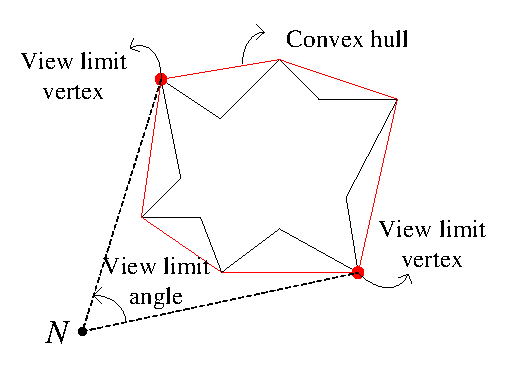
\includegraphics[width=0.6\textwidth]{Chapter4/Chapter4Figs/fig-view-limit-vertex.eps}
  \caption{View-limit vertices of $N$}
  \label{fig-def-viewlimit}
\end{subfigure}%
\begin{subfigure}{0.5\textwidth}
  \centering
  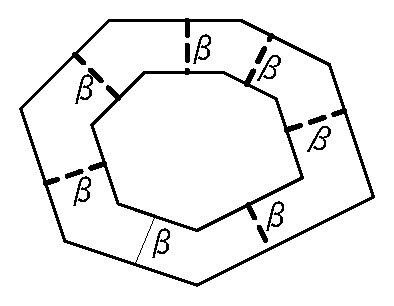
\includegraphics[width=0.6\textwidth]{Chapter4/Chapter4Figs/fig-covering-polygon.eps}
  \caption{$\beta$-covering polygon}
  \label{fig-def-betacovering}
\end{subfigure}
\caption{Illustrations of definition \ref{def-view-limit-vertex}, \ref{def-beta-covering}}
\label{fig-beta-covering}
\end{figure}

\begin{mydef}[$\beta$-covering]\label{def-beta-covering}
Assume that $P$ is a polygon and $\beta$ is a positive number. Then, $\beta$-covering polygon of $P$ is a polygon covering $P$ and having each edge parallels to an edge of $P$ while the distances between each parallel pair is the same $\beta$ (see Figure \ref{fig-def-betacovering}).
\end{mydef}

\begin{mydef}[Point-to-Polygon Distance]
Assume that $P$ is a convex polygon, $N$ is a point staying outside of $P$ . $d > 0$ is defined as the distance from $N$ to $P$ if and only if $N$ stays on the boundary of $d$-covering polygon of $P$.
\end{mydef}
The distance from point $N$ to polygon $P$ is denoted as $d(P, N)$.

\begin{mydef}[Inner polygon]
An inner polygon of polygon $P$ is a set of sequentially ordered nodes denoted by $IP_{P_{jk}} = \{ P_j, P_{j+1}, ..., P_k\}$, where $IP_{P_{jk}} \in P$ such that $P_j$ and $P_k$ are the extreme points of convex hull $C_P$. In particular, $P_jP_k$ is called the \textbf{gateway} of $IP_{P_{jk}}$.
\end{mydef}
Figure \ref{fig-def-inner} shows an example with four inner polygons and their gateways. There is a polygon $P$ (black edges). Polygon $P$ has four inner polygons which are $IP_1$, $IP_2$, $IP_3$, $IP_4$. The gateway of $IP_1$, $IP_2$, $IP_3$, $IP_4$ are $IP_{1_1}IP_{1_2}$, $IP_{2_1}IP_{2_2}$, $IP_{3_1}IP_{3_2}$, $IP_{4_1}IP_{4_2}$ (red edges), respectively.

\begin{figure}[!htb]
\centering
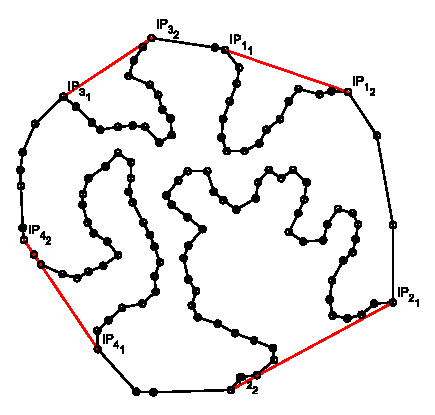
\includegraphics[width=0.3\textwidth]{Chapter4/Chapter4Figs/fig-innerpolygon.eps}
\caption{An example of inner polygons.}
\label{fig-def-inner}
\end{figure}

\subsection{Overview}
Our proposed scheme consists of two parts, namely the \emph{initial network setup} and the \emph{data forwarding}. The \emph{initial network setup} is designed to construct a graph for each inner polygon of the hole polygon. It consists of three phases: \emph{Hole Boundary Detection}, \emph{Hole Information Dissemination} and \emph{Internal Graph Construction}. Firstly, in the \emph{Hole Boundary Detection} phase, the hole boundary is identified using the \emph{BOUNDHOLE} algorithm \cite{boundhole}. During this phase, a leader node who is responsible for initiating the next phase: \emph{Hole Information Dissemination} is selected based on node IDs. This leader node also determines the convex hull of the hole polygon. Then, in the \emph{Hole Information Dissemination}, the hole polygon information is disseminated to the nodes surrounding the hole. The dissemination area is controlled by a system parameter $\delta$. The dissemination area is called the \textbf{near hole region}. Finally, in the \emph{Internal Graph Construction}, all nodes staying inside any inner polygons build an internal graph of its inner polygon. The internal graph is built based on the Voronoi diagram \cite{voronoi} of the inner polygon. It represents the internal structure of a inner polygon and is used for routing a packet optimally inside the convex hull of a hole.

Our data forwarding algorithm provides two routing mode, namely, \emph{near hole} mode and \emph{default} mode. The near hole routing consists of three cases:
\begin{itemize}
\item Both source node and destination node belong to the \emph{near hole region}.
\item Only source node belongs to the \emph{near hole region}.
\item Only destination node belongs to the \emph{near hole region}.
\end{itemize}

In the first case, the source node $s$ uses the \emph{near hole} mode to guide a packet out of the convex hull. If $s$ stays inside any inner polygons, it first finds an intermediate node in the \emph{gateway} and deliveries the packet to it. We call this intermediate node the source's \textbf{virtual anchor point} (VA-point). The detail algorithm to compute the VA-point is described in the next subsections. Otherwise, $s$ is the source's VA-point itself. In the source's VA-point, a \emph{dynamic forbidden area}, seen as a packet-specific forbidden area, is constructed. It is the image of the octagon covering the hole polygon through a homothetic transformation with the scale factor based on the distance from the source's VA-point to the convex hull. It also checks that if the destination node $d$ is inside any inner polygons. If the answer is ``yes'', it constructs the internal graph of the inner polygon containing $d$ and determines the destination's VA-point. The packet is then greedily forwarded to the VA-points which are the vertices of this packet-specific polygon. When the packet reaches the last VA-points, it is keeps greedily forwarding the packet to the destination's VA-point. Finally, the destination's VA-point forwards the packet to the destination based on the constructed internal graph. 
Figure \ref{fig-nhr-routing} shows an example of this case. In this figure, $I_s$ is the VA-point of the source node $s$, $I_1, I_2, I_3$ is the VA-points which are the vertices of scale octagon, and $I_d$ is the VA-point of the destination node $d$. The routing path is $\overrightarrow{sI_sI_1I_2I_3I_dd}$.

\begin{figure}[!htb]
\centering
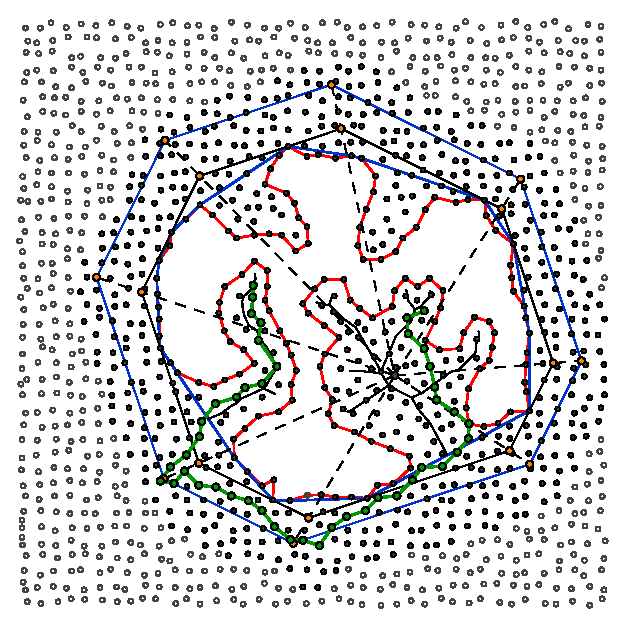
\includegraphics[width=0.4\textwidth]{Chapter4/Chapter4Figs/fig-path-example.eps}
\caption{An example of proposed routing path.}
\label{fig-nhr-routing}
\end{figure}

In the second case, the packet is forward along the routing path constructed same as the first case, until it reaches an intermediate node that does not belong to the \emph{near hole region}. Then the packet is greedily forwarded to destination node. In the third case, first, the packet is forward greedily to the destination, until it reaches an intermediate node belonging to the \emph{near hole region}. The routing path from this intermediate node to destination node is constructed same as the first case. In two later cases, the near hole routing protocol is used to find the path from the source to the intermediate node or from the intermediate node to the destination.

The detailed scheme is described in the following subsections.

\subsection{Hole Boundary Detection}
The \emph{TENT rule} is executed to identify the node on the hole boundary. Then, the \emph{Hole Boundary Detection} (\emph{HBD}) packet is formed and forwarded around the hole boundary using the \emph{BOUNDHOLE} algorithm. Assume $H_0$ is the leader node of the hole. After the \emph{HBD} packet came back to $H_0$, it has the information of all hole boundary sensor node $H_0, H_1, H_2, ..., H_n$. $H_0$ then uses the \emph{Graham scan} algorithm to determine the convex hull of the hole polygon. The information of each hole boundary sensor node is stored as format described in table \ref{table-node-info}.

\begin{table}[!htb]
\centering
\caption{Storage scheme of a hole boundary sensor node.}
\label{table-node-info}
\begin{tabular}{|l|l|}
\hline
x              & x-coordinate of node                                          \\ \hline
y              & y-coordinate of the node                                      \\ \hline
isExtremePoint & true if it is a vertex of the convex hull and false otherwise \\ \hline
\end{tabular}
\end{table}

\subsection{Hole Information Dissemination}
After the convex hull construction, node $H_0$ then creates a hole polygon information (\emph{HPI}) message that stores the information of the polygon vertices (which is the format described in table \ref{table-node-info}), and disseminates this \emph{HPI} message to its neighbors. In addition, to reduce the overhead of transmission information, before disseminating, $H_0$ will try to eliminate the vertices of any inner polygons whose vertices number is less than the system parameter $\eta$ (our experiments show that with an appropriately chosen value of $\eta$ (e.g., $\eta = 10$), it reduces the message overhead and still ensures the routing mechanism). This eliminating algorithm is described in algorithm \ref{alg-reduce-polygon}. 

\begin{algorithm}[!htb]
\SetAlgoLined
\caption{Hole polygon's vertices eliminating algorithm}
\label{alg-reduce-polygon}
\Input{$P = \{P_1, P_2, ..., P_n\}$: the linked list of the hole polygon vertices in counterclockwise order.\newline
$\eta$: pre-defined system parameter.}
\Output{$P$: simplified hole polygon.}
\For{$i = 1$ \KwTo $n$} {
	\uIf{$P[i].isExtremePoint = false$} {
		Remove $P[i]$ from $P$\;
		Append $P[i]$ to the end of $P$\;
	}
	\lElse {
		\KwBreak
	}
}
\For{$i = 1$ \KwTo $n$} {
	\If{$P[i].isExtremePoint = true$} {
		$j \leftarrow 0$\;
		$m \leftarrow i$\;
		\While{$P[i+1].isExtremePoint = false$} {
			$j \leftarrow j + 1$\;
			$i \leftarrow i + 1$\;
		}
		$i \leftarrow i - 1$\;
		\lIf{$j \leq \eta$} {
			Remove $\{P_{m+1}, P_{m+2}, ..., P_{i}\}$ from $P$
		}
	}
}
\Return $P$\;
\end{algorithm}

When an intermediate node $N$ receives this \emph{HPI} message, it does following tasks:
\begin{itemize}
\item Stores the information of the hole polygon to its local memory.
\item If $N$ is inside the convex hull of the hole polygon or its distance to the convex hull of hole polygon less than $\delta \times R_c$, it forwards the message to its neighbors.
\item Otherwise, it drops the message.
\end{itemize}
After this phase finished, the network is divided into two regions, and all the nodes that have hole information formed the \emph{near hole region}.

In addition, all sensor nodes also construct its \emph{core polygon} which is an octagon. This core polygon has to satisfy the following conditions:
\begin{itemize}
\item It completely covers the hole polygon.
\item It has at most 8 vertices and each edge of its contains at least one vertex of the hole.
\item All angles at the vertices that are not the vertices of the hole, equal to $\frac{3\pi}{4}$.
\end{itemize}
The reason for approximating the hole by an octagon is explained in subsection \ref{data-forwarding}. Algorithm \ref{algo-octagon-construction} describes how to construct the core polygon of specific node $N$.

\begin{algorithm}[!htb]
\SetAlgoLined
\caption{Core polygon construction algorithm}
\label{algo-octagon-construction}
\Input{$P=\left \{ P_1, ..., P_n \right \}$: the set of hole polygon vertices in counterclockwise order.\newline
$N$: current sensor node.}
\Output{$A = \{A_1, A_2, ..., A_8\}$: the core polygon of $N$.}
$P_j\leftarrow$ view-limit vertex of $N$ respect to $P$\;
$i \leftarrow 1$\;
$\alpha \leftarrow$ angle of $P_j$ with x-axis\;
$L \leftarrow \{P_jN\}$\;
\For{$k = 1$ \KwTo $n$} {
	$l \leftarrow$ line goes through $P_k$ and makes an angle of $\alpha + i \times \frac{\pi}{4}$ with x-axis\;
	\If{\emph{All hole polygon nodes stay on the left side of $l$}} {
		$L \leftarrow L \cup \{l\}$\;
		$i \leftarrow i + 1$\;
	}
	\lIf{$i > 8$} {
		\KwBreak
	}
}
\For{$k = 1$ \KwTo $8$} {
	$A_k \leftarrow L[k] \cap L[k+1]$\;
}
\Return $A$\;
\end{algorithm}


\subsection{Internal Graph Construction}
The most difficult part of building a near hole routing protocol is to find an optimal path for a packet to a destination node inside an inner polygon or from a source node inside an inner polygon to the outside of the convex hull. The \emph{Internal Graph Construction} phase is responsible for building an internal graph so that nodes are able to find such an optimal path. To ensure the requirements of a routing protocol that are load balancing and route stretch, this optimal path need to be as short as possible and is different for each sensor node. Our idea is to let every sensor node inside an inner polygon learn about the internal structure of that inner polygon via representing it by a \emph{skeleton}. This \emph{skeleton} is presented as a undirected acyclic graph, and it is built from the Voronoi diagram of the polygon without any Voronoi edges that does not inside the polygon. Figure \ref{fig-nhr-skeleton} shows an example of a \emph{skeleton}. 

\begin{figure}[!htb]
\centering
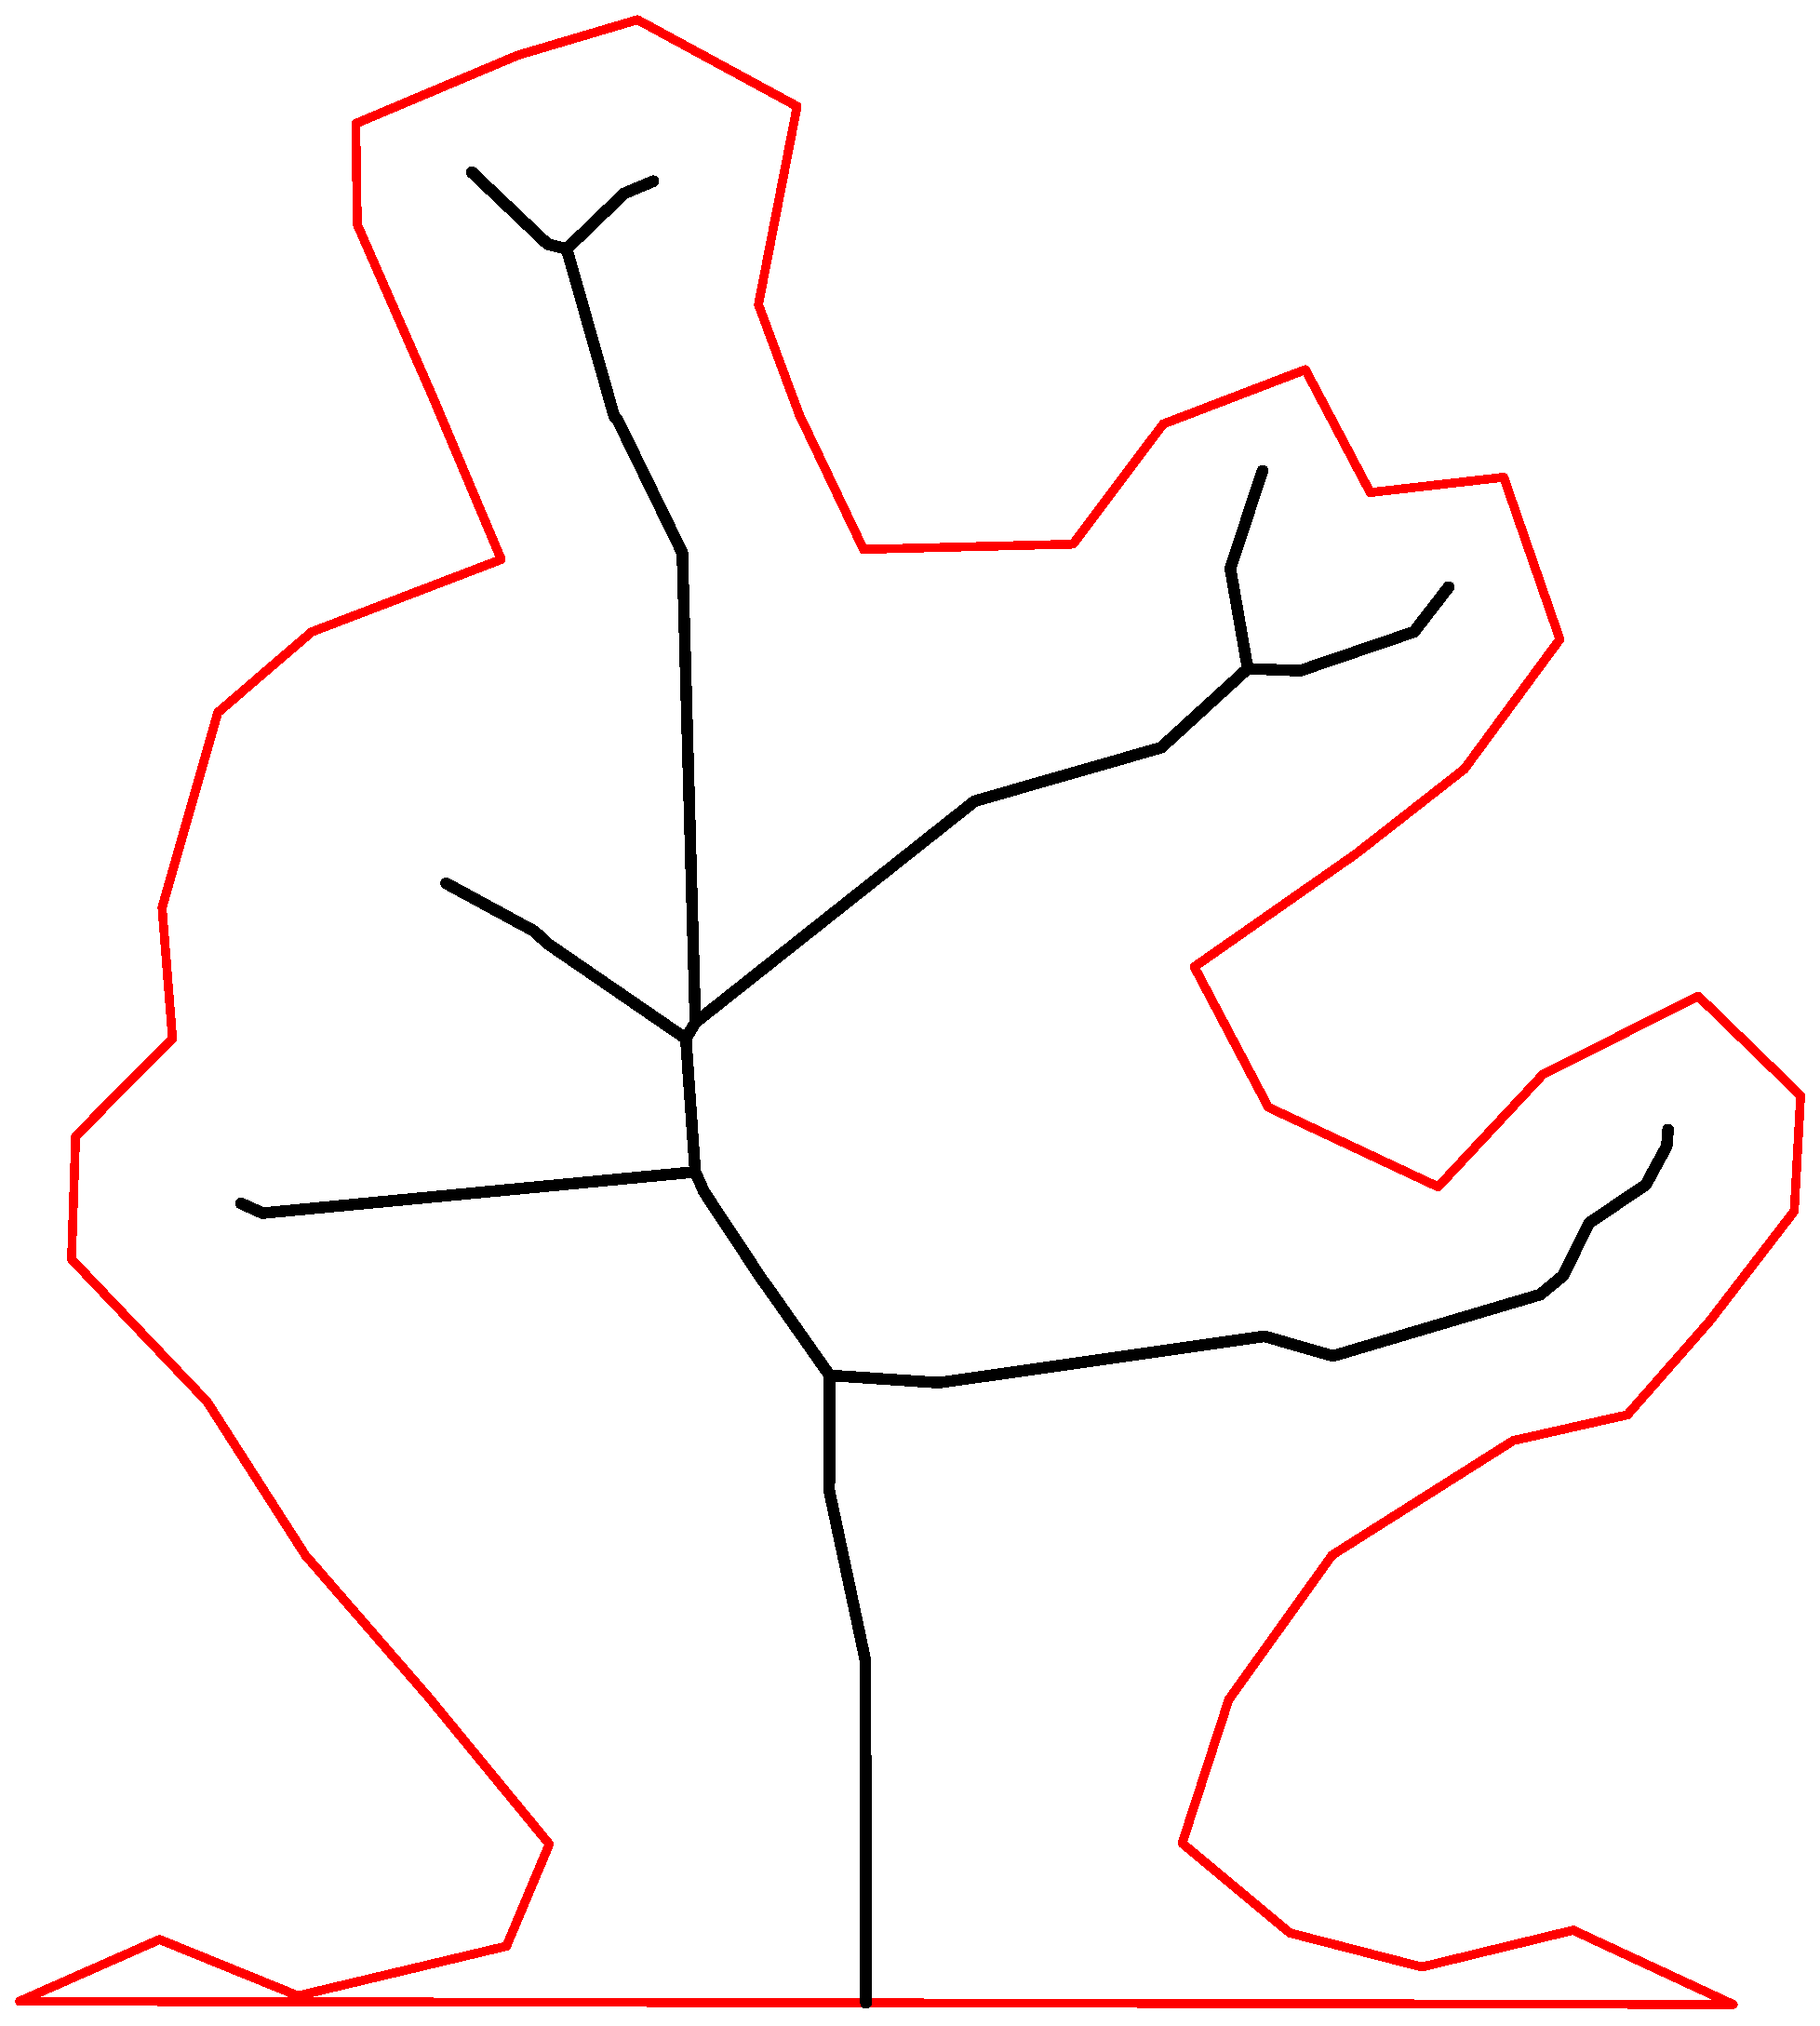
\includegraphics[width=0.4\textwidth]{Chapter4/Chapter4Figs/fig-skeleton.eps}
\caption{An example of polygon's skeleton.}
\label{fig-nhr-skeleton}
\end{figure}

Because this graph is calculated locally in each sensor node, node needs to know the location of only one point such that, if the packet is forwarded to that point, it still can find the way out the inner polygon by forwarding to the next point. We call such that point \textbf{endpoint}. On the other hand, from a point in the \emph{gateway}, we can re-construct the graph to find the way in from the gateway to the destination point. We call such that point \textbf{gate-point}. We also note that to reduce the node state, this graph is calculated only for each node to determine its \emph{endpoint}, and the nodes save the location of its \emph{endpoint} to its local memory, not the graph.
Algorithm \ref{algo-nhr-endpoint} describes how to construct such a skeleton and determine the \emph{endpoint} and \emph{gate-point} of a sensor node.

\begin{algorithm}[!htb]
\SetAlgoLined
\caption{Internal graph construction, endpoint and gate-point determination algorithm}
\label{algo-nhr-endpoint}
\Input{$N$: current sensor node}
\Output{$E_N$: endpoint of $N$\newline
$G_N$: gate-point of $N$}

\uIf{$N$ \emph{is not inside any inner polygons}} {
	$E_N \leftarrow N$\;
	$G_N \leftarrow null$\;
} 
\Else{
	$IP_{P_{hk}} \leftarrow$ inner polygon contains $N$\;
	$P_{h}P_{k} \leftarrow$ gateway of $IP_{P_{hk}}$\;
	$E_{IP_{P_{hk}}} \leftarrow$ set of edges of $IP_{P_{hk}}$\;
	$l \leftarrow$ perpendicular line from $N$ to $P_{h}P_{k}$\;
	$H \leftarrow l \cap P_{h}P_{k}$\;
	\uIf{$NH \cap \{E_{IP_{P_{hk}}} \setminus P_{h}P_{k}\} = \varnothing$}{
		$E_N \leftarrow H$\;
		$G_N \leftarrow null$\;
	}
	\Else {
		Construct Voronoi diagram $\upsilon$ of $IP_{P_{hk}}$\; 
		$\gamma \leftarrow$ Voronoi site contains $N$\;
		$V_j, V_{j+1}, ..., V_u \leftarrow$ Voronoi vertices of $\gamma$ inside $IP_{P_{hk}}$\;
		$K \leftarrow P_{i_h}P_{i_k} \cap e$ such that $e$ has a vertex inside $IP_{P_{hk}}$ and the other vertex outside $IP_{P_{hk}}$\;
		Eliminate all Voronoi edges not inside $IP_{P_{hk}}$ except $e$\;
		Construct graph from remaining edges\;
		Traversal the graph using BFS algorithm to find the shortest path from $V_j, V_{j+1}, ..., V_u$ to $K$\;
		$V_w\leftarrow$ is vertex corresponding to the shortest path among these paths\;
		$E_N \leftarrow V_w$\;
		$G_N \leftarrow K$\;
	}
}
\Return $E_N, G_N$\;
\end{algorithm}

By determining the \emph{endpoint} and \emph{gate-point} of a sensor node, we can route a packet to a destination node inside an inner polygon or route a packet from a source node inside an inner polygon to the outside of the convex hull. The details of this algorithm are presented in the next subsection. Note that this \emph{Internal Graph Construction} is performed only by nodes staying inside an inner polygon.

\subsection{Data Forwarding}
\label{data-forwarding}
In this subsection, we present the hole bypassing algorithm. As described above, the near hole routing path is constructed from VA-points. There are three type of VA-points: the source's VA-point, the VA-points which are vertices of scale octagon and the destination's VA-point. We use the octagon instead of the convex hull to reduce the number of VA-points' information stored in each packet, since the path constructed from the convex hull can contain a lot of VA-points and its number depends on the complexity of the convex hull. The routing path consists of three main periods: the first is from the source to its VA-point, the second is from the source's VA-point to the destination's VA-point and the last is from the destination's VA-point to the destination. Below we show how to determine these VA-points and the routing path of each period.

When a data packet is formed, the source node initiates its VA-point as its endpoint. The first period terminates immediately in case the source node is outside the convex hull. Otherwise, the packet is forwarded to this VA-point. At each intermediate node, the VA-point field is updated to the endpoint of current node. We note that the routing path inside the convex hull is different from each sensor node. It depends on the location of current sensor node, thus it still ensures the load balancing in inside the forbidden area. This period terminates when the packet reaches the \emph{gateway}. In case the source node does not belong to the \emph{near hole region}, it simply greedily forwards the packet the destination until it reaches an intermediate node belonging to the \emph{near hole region}.

Assume $I_s$ is this intermediate node. $I_s$ then uses its core polygon information $A$ to construct a scale polygon. This scale polygon is the image of core polygon $A$ through a homothetic transformation using a center $I$ chosen randomly inside the core polygon. The scale factor $\xi$ is computed based on the distance of $I_s$ to the convex hull and the system parameter $\delta$ as follows:\\
Let $d$ is maximum distance from $I$ to the vertices of $A$.
\begin{itemize}
\item $\xi = 1 + \frac{\delta \times R_c}{d}$ if $I_s$ is inside or on the edge of the convex hull
\item $\xi = 1 + \frac{d(C_P, I_s) \times R_c}{d}$ if $I_s$ is outside the convex hull 
\end{itemize}
$I_s$ also computes the destination's VA-point $I_d$ as follows:
\begin{itemize}
\item If the destination node $d$ is not inside any inner polygons, $I_d$ is the destination node.
\item Otherwise, $I_d$ is the \emph{gate-point} constructed from the internal graph of the inner polygon containing the destination node.
\end{itemize}

Then the algorithm \ref{algo-nhr-vap} is executed to determine VA-points which are vertices of scale octagon. Figure \ref{fig-nhr-vap} illustrates the algorithm.

\begin{figure}[!htb]
\centering
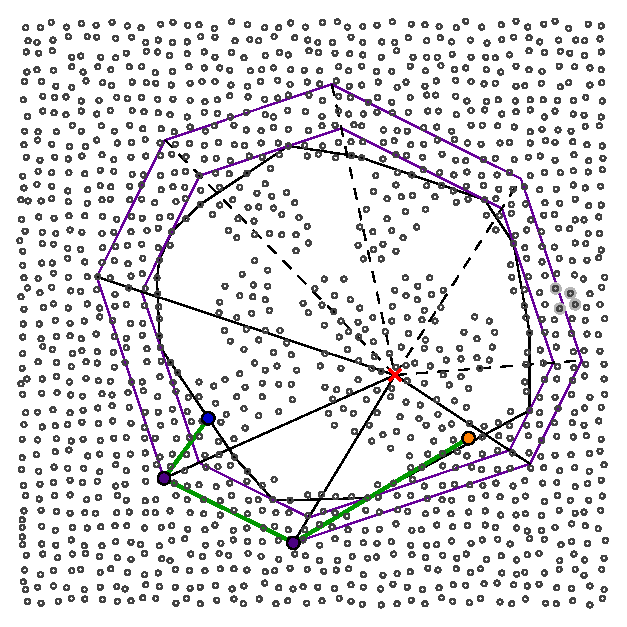
\includegraphics[width=0.4\textwidth]{Chapter4/Chapter4Figs/fig-octagon-vap.eps}
\caption{An example of choosing VA-points which are vertices of scale polygon.}
\label{fig-nhr-vap}
\end{figure}

\begin{algorithm}[!htb]
\SetAlgoLined
\caption{Virtual anchor points determination algorithm}
\label{algo-nhr-vap}
\nosemic Assume $I_s$ is current sensor node, $I_d$ is the destination's VA-point and $A' = \{A'_1, A'_2, ..., A'_m\}$ $(4 \leq m \leq 8)$ is the scale polygon with homothetic center $I$.\;
\nosemic Four points $L_s, L_d, R_s, R_d$ are computed as follows:\;
\uIf{$I_s$ is inside $A$}{
	$A'_i, A'_{i+1} \leftarrow$ two consecutive vertices of $A'$ such that $\bigtriangleup IA'_iA'_{i+1}$ contains $I_s$\;
	$L_s, R_s \leftarrow A'_i, A'_{i+1}$\;
}
\Else{
	$L_s, R_s \leftarrow$ view-limit vertices of $I_s$ respect to $A'$\;
}
\nosemic $L_d, R_d$ is computed same as $L_s, R_s$.\;
\nosemic Assume $L_s, L_s$ stay on the left side of $I_sI_d$ and $R_s, R_d$ stay on the right side of $I_sI_d$. The hole bypassing routing path is chosen as the shorter path between $\overrightarrow{I_sL_s...L_dI_d}$ and $\overrightarrow{I_sR_s...R_dI_d}$.
\end{algorithm}
The information of virtual anchor points is added to the packet header. The packet then is forwarded greedily to each virtual anchor point. 

In the last virtual anchor point, i.e. the destination's VA-point, it re-construct the internal graph of the inner polygon containing the destination in case the destination is inside an inner polygon, or it simply use the greedy protocol to forward the packet to the destination. If the destination is inside an inner polygon, the internal graph construction is performed in some specific nodes, that are the Voronoi vertices of the graph, not all the nodes in the routing path. In this process, the BFS algorithm is executed to trace back the shortest path from the \emph{gate-point} to the destination node. This process terminates when the packet reaches the \emph{endpoint} of the destination node.

Algorithm \ref{algo-nhr} presents the hole bypassing protocol.

\begin{algorithm}[!htb]
\SetAlgoLined
\caption{Hole bypassing protocol.}
\label{algo-nhr}
\Input{$N$: current sensor node\newline
$D$: destination node\newline
$AP$: the set of virtual anchor points\newline
$i$: current index of $AP$}
\Output{$next$: the location of the next hop}
Assume $getNextHopByGreedy(N, D$ returns the neighbor of $N$ which is nearest to $D$\;
$period \leftarrow$ current routing period\;
\If{$period = 1$}{
	$I_d \leftarrow$ endpoint of $N$\;
	$AP[6] \leftarrow I_d$\;
	$i \leftarrow 6$\;
}
\uIf{$N$ is a virtual anchor point}{
	$i \leftarrow i -1$\;
}
\ElseIf{$N$ is its endpoint}{
	$A \leftarrow$ core polygon\;
	$A' \leftarrow$ scale polygon\;
	$A'_1, A'_2, A'_3, A'_4 \leftarrow$ virtual anchor points computed from $A'$\;
	$AP[2..5] \leftarrow A'_1, A'_2, A'_3, A'_4$\;
	$i \leftarrow 5$\;
	% $I_s \leftarrow$ 
}
$next \leftarrow getNextHopByGreedy(N, AP[i])$\;
\Return $next$\;
\end{algorithm}

\section{Theoretical Analysis}
% \subsection{Validity of the protocol}
\subsection{Impact of parameter $\delta$ over the protocol}
The value of $\delta$ decides the area of the near hole region. The greater the value of $\delta$ is, the bigger the near hole region is. In the following, We show that the area of near hole region has a big impact on the two factors: energy consumption of the network and route stretch.

In case $\delta$ is big, the are of near hole region is big. Thus, the \emph{HPI} message is broadcast further, and more. Consequently, the energy consumption of the network increases. If $\delta$ is small, the \emph{HPI} message is broadcast lesser. Hence, the energy consumption of the network decreases.

In addition, if $\delta$ is small, the scale factor of the homothetic transformation is small. It makes all scale octagons almost the same. With a randomly deployed network, the density of sensor nodes is not really high, this would not create different routing path for different scale octagon. Thus, it decreases the load balancing. Vice versa, if $\delta$ is big, the scale factor is big, the virtual anchor points are far from the core polygon. It leads to the path enlargement problem.

According to mentioned analysis, obviously, the value of $\delta$ affects load balancing, energy consumption as well as route stretch. We also conducted experiments to prove these analysis and give a conclusion on the appropriate value of $\delta$.
